\documentclass[a4paper]{article}

%% Language and font encodings
\usepackage[english]{babel}
\usepackage[utf8x]{inputenc}
\usepackage[T1]{fontenc}

%% Sets page size and margins
\usepackage[a4paper,top=3cm,bottom=2cm,left=3cm,right=3cm,marginparwidth=1.75cm]{geometry}

%% Useful packages
\usepackage{amssymb}
\usepackage{amsmath}
\usepackage{graphicx}
\usepackage{subfigure}
\usepackage{caption}
\usepackage{float}

\usepackage[colorinlistoftodos]{todonotes}
\usepackage[colorlinks=true, allcolors=blue]{hyperref}

\title{
Simulated Annealing for the Ising perceptron \\
Markov Chains and Algorithmic Applications project}

\author{
Nicolas Roussel\\
EPFL}

\begin{document}
\maketitle

\begin{abstract}
In this report, we formulate the Ising perceptron in a learning problem and use a Markov Chain Monte-Carlo (MCMC) method to solve it. In particular, the simulated annealing algorithm will be used to avoid local minimums and improve the convergence speed. This report will recall the problem statement and describe several simulated annealing schemes with their respective results.\end{abstract}

\section{Problem statement}

Let $\underline{w}^*$ be a random vector of size $N$ where every component is in \{-1, +1\} (i.i.d. uniformly distributed). This vector is the goal weights to achieve by our Ising perceptron. We then generate \textit{M} vectors of size \textit{N} which we call $\underline{x}_{\mu}$ for $\mu = 1, 2, .., M$ such that $\underline{x}_{\mu} \in \mathbb{R}^{N}$. These are the patterns of the dataset. Finally, from these patterns and weights we generate $y_{\mu}$ where
\[y_{\mu} = sign(\underline{w}^* \cdot \underline{x}_{\mu}) \;, \;\mu = 1, 2, .., M\]
This is a vector of size $M$ where each of its components is respectively the class assigned to $\underline{x}_{\mu}$.

The goal of the problem is to find $\underline{w}^*$ when only given the pattern and classes pairs ($\underline{x}_{\mu}$, $y_{\mu}$). Note that we define $M$ as $\alpha = M/N$, and are interested in the different values $\alpha$ can take for large $M, N$.  

\section{MCMC solution}\label{MCMC_SOL}

The Markov Chain Monte-Carlo solution to this problem is quite straightforward. The core idea is to start from a random weights vector $\underline{w}$ and swap its components until we reach a solution to the following equation: 
 \[y_{\mu} = sign(\underline{w} \cdot \underline{x}_{\mu}) \;, \;\mu = 1, 2, .., M\]
 
 Here is the actual algorithm step by step:
 
\begin{enumerate}
\item Start from a random initial vector $\underline{w} \in \{-1, +1\}^{N}$
\item Compute the current energy of this weights vector as $E(\underline{w}) = \frac{1}{2} \sum_{\mu = 1}^{M} (y_{\mu} - sign(\underline{w} \cdot \underline{x}_{\mu}))^2$
\item Select uniformly a component of $\underline{w}$ and swap its sign (from -1 to 1 or 1 to -1). Call this vector $\underline{w}'$.
\item Compute the energy of $\underline{w}'$ as in step 2. 
\item Accept $\underline{w}'$ as the current weights vector  $\underline{w}$ with probability \[a_{\beta}(\underline{w}, \underline{w}') = min(1, exp(-\beta(E(\underline{w}') - E(\underline{w}))))\] $\beta$ is called the temperature parameter (assume that it is a fixed scalar for now).
\item Iterate steps 2 through 5 until $E(\underline{w})$ is sufficiently low.
\end{enumerate}

\section{Simulated annealing}

In the previous solution the $\beta$ parameter is fixed. However, by changing this parameter as we iterate we might converge faster or even get a better result depending on how these changes are done. The intuition here is to start with a small temperature and increase it as we go, this will guarantee that when $\beta$ is very high there will be no more changes accepted as according to the acceptance formula in step 5.
There are obviously a lot of different temperature increasing schemes possible, we will from now on refer to them as temperature schedules, or just schedules. For example, we could simply linearly increase $\beta$ at each iteration.

\section{Results}
\subsection{First part: constant schedules}

Constant schedules are exactly the algorithm described in chapter \ref{MCMC_SOL}, the temperature $\beta$ remains constant throughout the whole algorithm.

\begin{figure}[!htb]
 \centering
\minipage{0.8\linewidth}
\centering
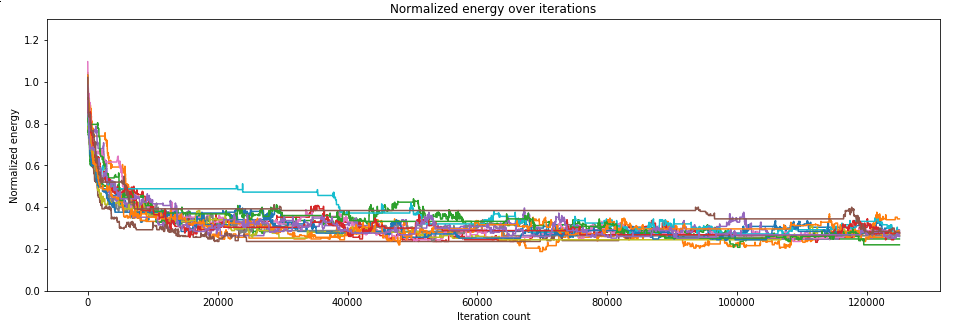
\includegraphics[width=1.0\textwidth]{FIG1.png}
\caption{\label{fig:FIG1}Normalized energy over iterations for $\beta = 0.6$, $\alpha = 2$ and $N = 250$. The colors are 16 independent runs of the algorithm.}
\endminipage\par\medskip
\minipage{0.49\linewidth}
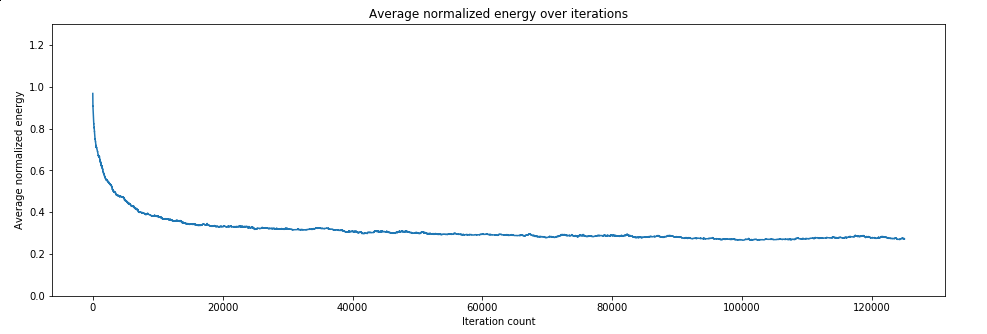
\includegraphics[width=1.0\textwidth]{FIG2.png}
\caption{\label{fig:FIG2}Averaged normalized energy over iterations for $\beta = 0.6$, $\alpha = 2$ and $N = 250$. Averaged over 16 independent runs of the algorithm.}
\endminipage\hfill
\minipage{0.49\linewidth}%
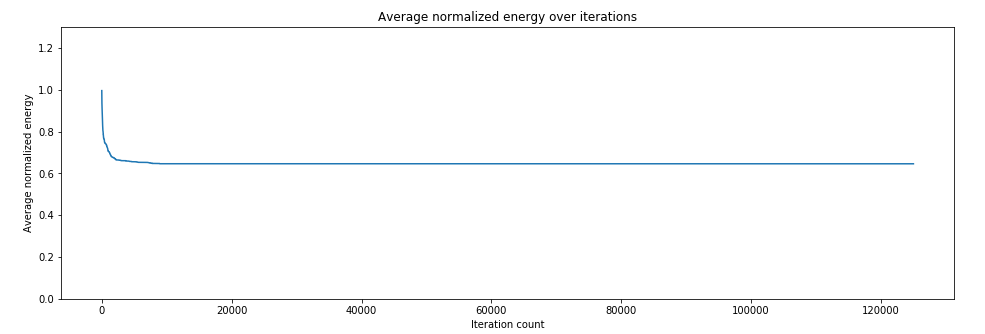
\includegraphics[width=1.0\textwidth]{FIG3.png}
\caption{\label{fig:FIG3}Averaged normalized energy over iterations for $\beta = 4$, $\alpha = 3.5$ and $N = 250$. Averaged over 16 independent runs of the algorithm.}
\endminipage
\end{figure}


Figure \ref{fig:FIG1}, \ref{fig:FIG2} and \ref{fig:FIG3} illustrate how the energy typically evolves over time for a constant schedule (other values of $\alpha$ and $\beta$ show the same behavior). The main difference which can be observed when changing $\alpha$ and $\beta$ is how fast the energy plateaus and at which value. Figure \ref{fig:FIG2} and \ref{fig:FIG3} illustrates this. When $\beta$ is very small, the plots are much noisier and the normalized energy typically stays around 1. This happens due to the fact that the acceptance probability is always 1 or close to 1.

Another metric is the overlap $q(\alpha, \beta) = \frac{1}{N} \sum_{i = 1}^{N}(w_i w_{i}^{*})$. This indicates how close we are to the ground truth weights (our goal). For cases where $\alpha$ is small there might be several solutions to the equation in chapter \ref{MCMC_SOL}, hence the energy can reach 0 but the overlap is not 1.

Figures \ref{fig:FIG4} and \ref{fig:FIG5} respectively show the averaged normalized energies and overlaps as function of $\alpha$ for different values of $\beta$. Interestingly enough we can see the performance completely switch order as $\alpha$ grows.

This can be explained by the previously mentioned case where the acceptance probability is very close to 1 - when both $\alpha$ and $\beta$ are small. Additionally, as said before, when $\alpha$ is small there are multiple weight vectors which can reach a very low energy but might not have a good overlap. This is exactly what is illustrated in both figures.

\begin{figure}
\centering
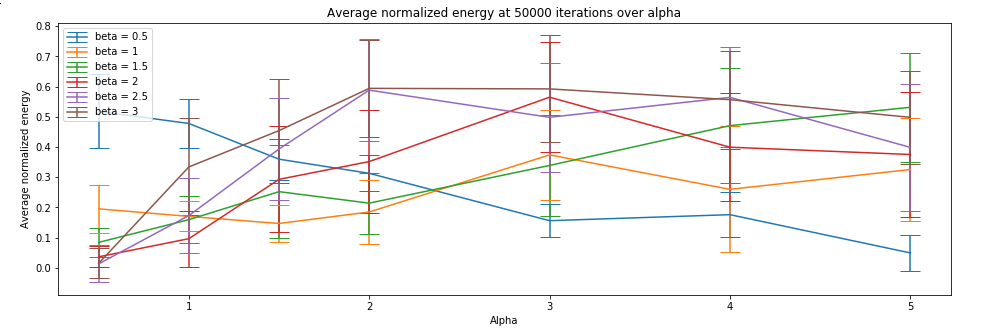
\includegraphics[width=0.9\textwidth]{FIG4.png}
\caption{\label{fig:FIG4}Averaged normalized energy at 50000 iterations over $\alpha$ for $N = 100$. Averaged over 128 independent runs of the algorithm. The horizontal caps represent the standard deviation of the measures.}
\end{figure}


\begin{figure}
\centering
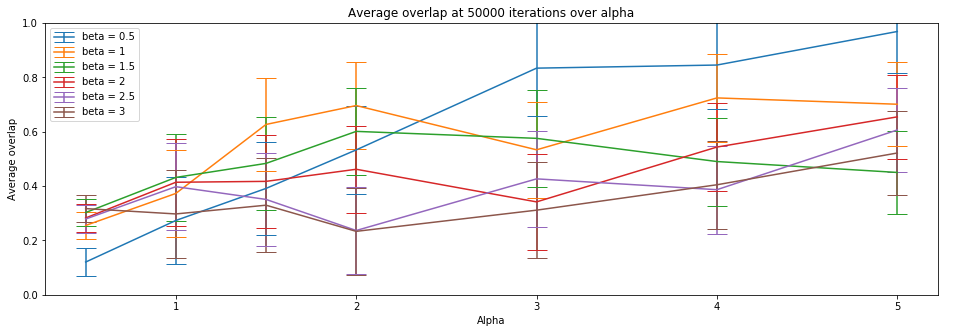
\includegraphics[width=0.9\textwidth]{FIG5.png}
\caption{\label{fig:FIG5}Averaged overlap at 50000 iterations over $\alpha$ for $N = 100$. Averaged over 128 independent runs of the algorithm. The horizontal caps represent the standard deviation of the measures.}
\end{figure}

\subsection{Second part: linear, polynomial, logarithmic and exponential schedules}

These are the schedules which were experimented with : linear, sublinear, polynomial, logarithmic and exponential. The Figure \ref{fig:FIG6} illustrates each one of them and the Table \ref{table:TAB1} has their formal definitions. They were all optimized with a coarse grained grid search for $N = 100$, and $\alpha = 5$. Of course, there might be added value to optimizing these parameters for individual $\alpha$s and $N$s.

There was also an experiment to quantize these schedules. The main difference would be that the temperature would not change at every iteration, but only after a few iterations. There was no signifcant improvement to notice.

Figure \ref{fig:FIG7} and \ref{fig:FIG8} show the average normalized energies and overlaps of each schedule.

\begin{center}
\begin{table}[H]
\begin{tabular}{ |c|c|c|c|c|c|} 
\hline
\textbf{Constant} & \textbf{Linear} & \textbf{Sublinear} & \textbf{Polynomial} & \textbf{Logarithmic} & \textbf{Exponential} \\
\hline
$\beta_0$ & $\beta_0$ + $\gamma t$ & $\beta_0 t^{\gamma}, \gamma < 1$ & $\beta_0 t^{\gamma}, \gamma > 1$  & $\beta_0 \log(t + \gamma), \gamma > 1$ & $\beta_0 \gamma^{-t}, 0 <\gamma < 1$  \\ 
$\beta_0 = 0.6$ & $\beta_0 = 0.2$ & $\beta_0 = 1.1$ & $\beta_0 = 1.1$ & $\beta_0 = 1.1$ & $\beta_0 = 0.15$ \\ 
  & $\gamma = 0.7$ & $\gamma = 0.8$ & $\gamma = 1.5$ & $\gamma = 01.2$ & $\gamma = 0.1$ \\ 
\hline
\end{tabular}
\caption{Schedule definitions where $t$ is the fraction of total iterations to complete.}
\label{table:TAB1}
\end{table}
\end{center}

\begin{figure}
\centering
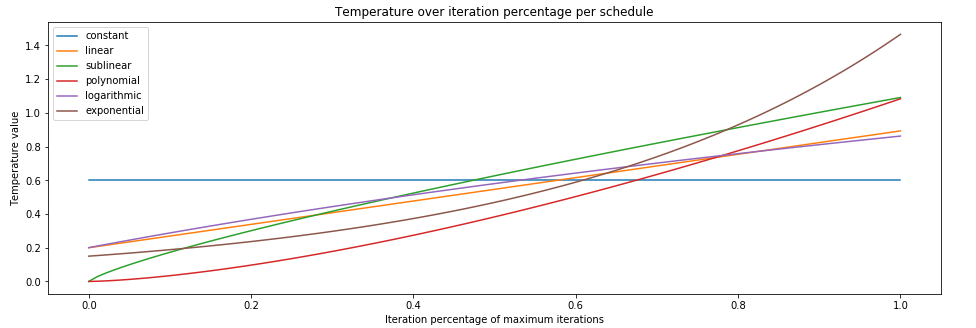
\includegraphics[width=1.0\textwidth]{FIG6.png}
\caption{\label{fig:FIG6}Temperature schedules}
\end{figure}

\begin{figure}
\centering
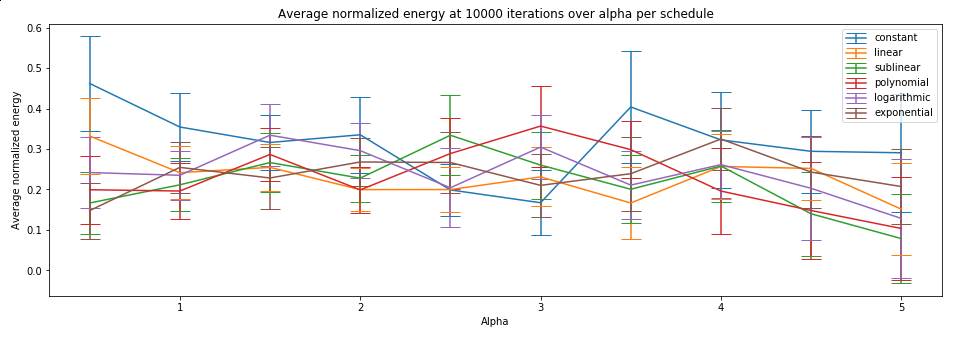
\includegraphics[width=1.0\textwidth]{FIG7.png}
\caption{\label{fig:FIG7}Average normalized energy at 10000 iterations over $\alpha$ per schedule ($N = 100$). Averaged over 128 independent runs of the algorithm. The horizontal caps represent the standard deviation of the measures.}
\end{figure}

\begin{figure}
\centering
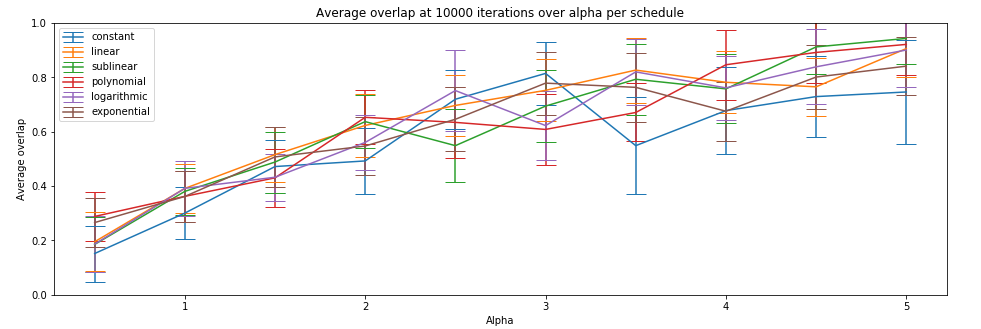
\includegraphics[width=1.0\textwidth]{FIG8.png}
\caption{\label{fig:FIG8}Average ovlerap at 10000 iterations over $\alpha$ per schedule ($N = 100$). Averaged over 128 independent runs of the algorithm. The horizontal caps represent the standard deviation of the measures.}
\end{figure}

\section{Conclusion}
There is no schedule which has a clear advantage over all others. However, slow-growing functions do have a better standard deviation which make them more consistent in practice. Differences might be more marked with larger values for $N$ and better tuned parameters - more computation time would be needed.

\section{Going further}
There are a few more steps one can take to improve the performance of the final schedules found here. First of all, some finer tuning of the schedule parameters might give better results. Adding a constant offset to the temperature for certain schedules would avoid acceptance probabilities close to 1 in early stages of the algorithm. Investigating into other schemes might also be an interesting path to take, there might be parts of the schedule which can be more "aggressive" in their increases. Finally, using a Gibbs sampler instead of a Metropolis approach to this simulated annealing problem could also give some additional insights.

\end{document}
